\documentclass[conference]{IEEEtran}
\IEEEoverridecommandlockouts
% The preceding line is only needed to identify funding in the first footnote. If that is unneeded, please comment it out.
\usepackage{cite}
\usepackage{amsmath,amssymb,amsfonts}
\usepackage{algorithmic}
\usepackage{graphicx}
\usepackage{textcomp}
\usepackage{hyperref}
\usepackage{listings}
\usepackage{xcolor}
\usepackage{listings}
\usepackage{caption}
\usepackage{subcaption}
\usepackage{minted}
\def\BibTeX{{\rm B\kern-.05em{\sc i\kern-.025em b}\kern-.08em
    T\kern-.1667em\lower.7ex\hbox{E}\kern-.125emX}}
\begin{document}
\lstset{
breaklines=True
}
\title{BREAST CANCER PREDICTION USING MACHINE LEARNING}

\author{
\IEEEauthorblockN{BHUVANA KORRAPATI}
\IEEEauthorblockA{\textit{Department of Computer Science} \\
\textit{University of North Carolina at Greensboro}\\
Greensboro, USA \\
bkorrapati@gmail.com}
}

\maketitle

\begin{abstract}
Breast cancer is the leading cause of mortality from cancer for women between the ages of 20 and 59 and the second leading cause for women over the age of 59. To stop the disease's progression and lower its morbidity rates, it is crucial to diagnose and treat this pathology as soon as possible. Several factors are considered for the accurate prediction of the cancer such as radius, texture, compactness, concavity. So this paper presents the detail description of the features and prediction of the stroke using two different algorithms that are Support Vector Machine(SVM) and Convolution neural networks(CNN).
\end{abstract}

\section{Introduction}
The most prevalent illness in women is diagnosed as breast cancer. Every year more than 2.23 million women are diagnosed with the breast cancer.  In this project we analyse the sample data that is collected from UCI macine learning dataset repository[1]. The machine learning algorithms that is Support Vector Machine(SVM) and Convolution neural network(CNN) are  used to analyse and predict the dataset. The predicted values should be highly accurate to diagnose the disease, since the comparison between the algorithms are made. CNN provides the higher accuracy comparitively for the given dataset.   
\section{Setting up Environment}
Mostly python or R language is used for the machine learning programming. Anaconda environment was downloaded from the official Anaconda website[2] and for proper installation followed the steps mentioned in the website[3]. Python provides access to large number of libraries and frameworks. Anaconda is a free open-source environment which consists of over 250 automatically installed packages.
For the programming, jupyter notebook is installed with all the necessary packages and used for the code description, prepossessing and algorithm application to the given dataset. The libraries to run scikit-learn and TensorFlow is installed in the jupyter notebook.

\begin{figure}[h]
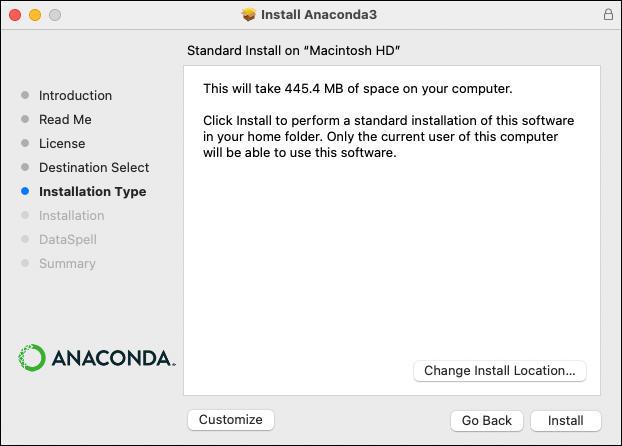
\includegraphics[width=.24\textwidth]{osx.png}\hfill
\includegraphics[width=.24\textwidth]{juy.png}\hfill
\caption{Left: anaconda for mac. Right:anaconda installation.}
\end{figure}

\section{Dataset Description}
The dataset that is considered for the prediction of the cancer consists of the features such as diagnosis, radius, texture, perimeter, area, smoothness, compactness, concavity. These are the dimensional measure of the tumor. All the mean values, worst values are considered. Here the compactness represents the volume of the tumor, concavity represents the concave positions. The labels that is 'M' represents the malignant tumor and 'B' represents the benign tumor. Malignant is the  process in which the cancer cells are multiplied and are harmful, finally leads to the cancer. Benign is a standard tumor where this is not harmful and cannot spread the cancer cells.
\begin{figure}[h!]
    \centerline{\includegraphics[width=5cm,height=4cm]{on.png}}
    \caption{diagnosis count}
\end{figure}
\section{Data Preprocessing}
The data can be considered as three parts that is number of observations, features and the labels. The number of observations are considered to be the total instances. The "features" that make up a data set used to describe or communicate the data set itself. This may depend on factors including size, location, age, time, color, etc. Features are sometimes referred to as attributes, variables, fields, and characteristics. They appear as columns in datasets. The label is to differentiate the classes and is only observed in supervised machine learning models. 
The data can be imbalanced, inaccurate or incorrect, by some simple statistical approaches we can clean the noise data. the processing of the data includes identifying and dropping unnecessary columns or features, detect null values and fill it with the mean or median values as this can cause bias for data processing.we can even describe the data and check the values for each feature and find the correlation as well.
\begin{figure}[h!]
    \centerline{\includegraphics[width=5cm,height=4cm]{one.png}}
    \caption{correlation heatmap}
\end{figure}
\section{Proposed Methodology}
Machine Learning algorithms are used for the classification and prediction of the data, The dataset is divided by 80:20 rule that is 80 percent of training data and 20 percent of testing data. It is a proven rule to split the dataset for better accuracy as well and to reduce the problem of non seen data. The training and testing datasets are saved as a csv files. 

\begin{figure}[h!]
    \centerline{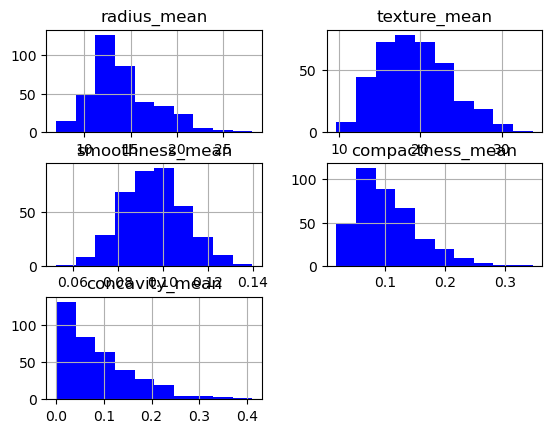
\includegraphics[width=5cm,height=4cm]{gra.png}}
    \caption{Training data graphs}
\end{figure}
\begin{figure}[h!]
    \centerline{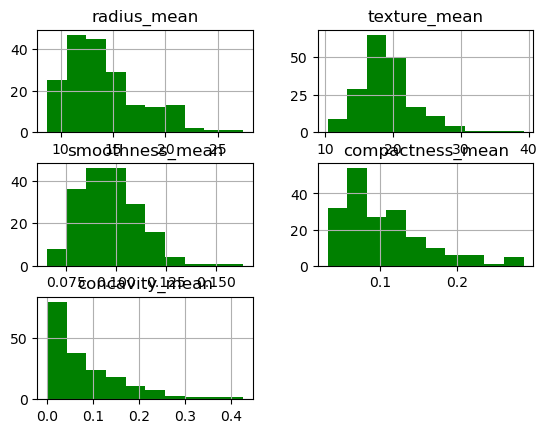
\includegraphics[width=5cm,height=4cm]{graa.png}}
    \caption{Testing data graphs}
\end{figure}

\subsection{SVM CLASSIFICATION}
The support vector machine is a supervised machine learning algorithm. This is the mathematical model where the input data is not scalable. The data cannot get added after the data is trained. We use C-Support Vector Classification to classify this dataset. The steps includes importing the library and calling the function to perform the svm model.\\

Table.1.\\
\begin{table}[h]
\centering
\begin{tabular}{ | c | c | }
 \hline
 Our Accuracy Score  & 0.925531914893617 \\
 \hline
 Our Precision Score  & 0.9090909090909091 \\
 \hline
 Our Sensitivity Score & 0.9836065573770493 \\
 \hline
 Our Specificity Score & 0.8181818181818181 \\
 \hline
\end{tabular}
\caption{SVM Quaility Measures}
\end{table}

\subsection{Convolution Neural Networks}
The CNN is a deep learning algorithm. This is the hierarchical model where the input data is scalable. The data cannot get added after the data is trained. We use C-Support Vector Classification to classify this dataset. The steps includes importing the library and calling the function to perform the CNN model.

\begin{figure}[h]
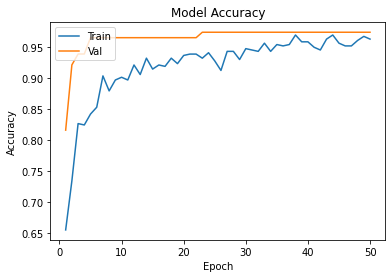
\includegraphics[width=.24\textwidth]{im.png}\hfill
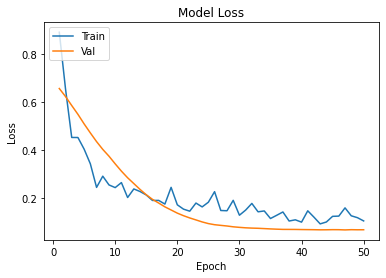
\includegraphics[width=.24\textwidth]{ima.png}\hfill
\caption{Left: anaconda for mac. Right:anaconda installation.}
\end{figure}


\begin{figure}[h!]
    \centerline{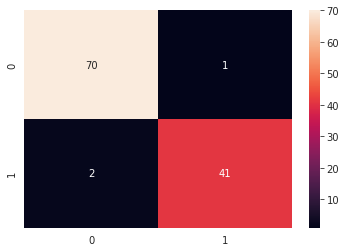
\includegraphics[width=5cm,height=4cm]{con.png}}
    \caption{confusion matrix}
\end{figure}

Table.1.\\
\begin{table}[h]
\centering
\begin{tabular}{ | c | c | }
 \hline
 Our Accuracy Score  & 0.9736842105263158 \\
 \hline
 Our Precision Score  & 0.9761904761904762 \\
 \hline
 Our Sensitivity Score & 0.9534883720930232 \\
 \hline
 Our Specificity Score & 0.9859154929577465 \\
 \hline
\end{tabular}
\caption{CNN Quaility Measures}
\end{table}
\section{Conclusion}
According to the performance evaluation of both the algorithms, both CNN and SVM classifiers achieve comparable results. CNN is even scalable with different epochs and batch range. We can add the new data when ever available as it is one observation training. Comparatively CNN has high accuracy and precision values and is recommended in this case.

\section{References}
\begin{thebibliography}{00}
\bibitem{b1} http://archive.ics.uci.edu/ml/machine-learning-databases/breast-cancer-wisconsin/ 
\bibitem{b2} https://docs.anaconda.com/anaconda/
\bibitem{b3} https://www.anaconda.com/products/individual
\bibitem{b4} https://scikit-learn.org/stable/install.html
\bibitem{b5}https://scikitlearn.org/stable/modules/generated/sklearn.svm.SVC.html?highlight=svm

\end{thebibliography}
\vspace{12pt}
\end{document}
